%\newpage

\begin{center}
\subsection*{ОСНОВНОЕ СОДЕРЖАНИЕ РАБОТЫ}
\end{center}

Во {\textbf{введении}} обосновывается актуальность исследований, на основании чего сформулированы цель и задачи работы; определены объект, предмет, методы и средства исследования; раскрыта научная новизна и практическая значимость полученных результатов; изложены основные научные положения, выносимые на защиту; приведены структура и краткий обзор содержания работы.

В \textbf {первой главе} анализируются алгоритмический подход, методы компьютерного зрения в извлечении антропометрических признаков со статических изображений и видеопоследовательностей: Построение признаков ключевых точек из 2D-изображений, видеокадров; Использование 3D-сканирования моделей и сопоставление точек человеческого тела в построенных моделях.

В данной главе анализируется алгоритмический подход, методы компьютерного зрения в классификации антропометрических данных признаков в изображениях и видеопоследовательностях. Включая: Алгоритм Adaboost; Нейронные сети; Опорных векторов (SVM).

Также здесь рассматриваются возможности использования алгоритмов ICP и разреза на графах (Graph-сuts) для извлечения антропометрических признаков и алгоритм случайного леса для классификации антропометрических данных в изображениях и видеопоследовательностях.

На основе проведенного анализа принято решение о адекватности и точности использования комбинированных алгоритмов ICP, разреза на графах (Graph-cuts) для извлечения антропометрических признаков с использованием метода случайного леса (Random Forest) для классификации антропометрических данных в статических изображениях, видео в присутствии шума и в режиме реального времени. Такой подход позволяет построить систему компьютерного зрения в антропометрии с высокой точностью и скоростью обработки.

Во \textbf{второй главе} излагаются принципы решения проблем приложения компьютерного зрения в задаче антропометрии использую статические изображения или видеопоследовательностях в режиме реального времени. Приводится подробное описание алгоритмов и методов, используемых для обнаружения и классификации объектов, извлечения признаков на изображениях и видеопоследовательностях.

Целью работы была разработка автоматизированной измерительной системы, основанной на изображениях и видео на смартфоне. Эта система использует методы и алгоритмы обработки изображений и машинного обучения компьютерного зрения.
Наша система состоит из трех основных частей: извлечение антропометрических признаков, процессы обучения и тестирования, классификация новых данных (рис. \ref{img7}). Новизна нашего подхода заключаются в следующих пунктах: Классификация антропометрических признаков на основе алгоритмов машинного обучения; Разработка программного комплекса бесконтактной антропометрии для смартфона; Создание 3D-модели человеческого тела на основе полученных антропометрических признаков.

\textbf {Алгоритм извлечения антропометрических признаков из видео}. Для решения задачи извлечения антропометрических признаков с изображения и видео предложен алгоритм, основанный на  комбинации новейших методов - технике предварительной обработки изображений, алгоритме вычитания фона, алгоритме сегментации изображений на основе разреза на графах, алгоритме итеративных ближайших точек. В этом алгоритме, человек рассматривается как объект и появляется на картине. Процесс извлечения антропометрических признаков объектов на изображении и видео на основе алгоритма компьютерного зрения включает в себя следующие этапы:

\textbf{Шаг 1:} Предварительная обработка изображения;
Вначале происходит преобразова-ние входного изображения из формата RGB в полутоновое изображение. Предварительная обработка и нормализация изображения: на этапе необходимо выполнить фильтрацию шума и сглаживание изображения, применить морфологические операторы для улучшения качества контура объекта, использовать уравнивания гистограммы, чтобы сбалансировать яркость, контраст в условиях низкой освещенности для системы захвата изображений, видео с хорошим качеством.

\textbf{Шаг 2:} Обнаружение объектов. На основе фотографий с помощью модели, основанной на алгоритме вычитания фона. Основная идея алгоритма вычитания фона моделью следующая. Пиксель в положении в изображении принадлежит доминирующая компонента, если он удовлетворяет неравенству: $\left|I_n\left(x\right)-B_n\left(x\right)\right| \geq T_n\left(x\right)$. Здесь $ I_n\left(x\right) \in \left[0,255\right]$- значение интенсивности серого в позиции пикселя x принадлежит $n$-му изображению или видеофрагменту; $B_n \left(x\right)$  - значение интенсивности фона в местоположении пикселя $x$; $T_n \left(x\right)$  - пороговое значение задается для каждого изображения. Модель базового фона постоянно обновляется из исходных изображений или видео по формула: $B_{n+1}\left(x\right)= \left\{\begin{array}{l} \alpha B_n\left(x\right)+\left(1-\alpha\right)I_n\left(x\right),x\in BG,\\
\beta B_n\left(x\right)+\left(1-\beta\right)I_n\left(x\right),x\in FG,
\end{array}\right.$; $T_{n+1}\left(x\right)= \left\{\begin{array}{l} \alpha T_n \left(x\right)+\left(1-\alpha\right) \left(\left|I_n\left(x\right)-B_n\left(x\right)\right|\right), x \in BG,\\
T_n\left(x\right), x\in FG,
\end{array}\right.$

\textbf{Шаг 3:} Сегментация изображения алгоритмом разреза на графах. Поиск области изображения, содержащего части тела человека на основе формулы определения энергии пикселей $E\left(f\right) = \sum_{p \in P}D_p\left(f_p\right)+\sum_{p,q \in N}V_{p,q}\left(f_p,f_q\right)$. Найти маркировки $f:P\rightarrow L$ , что сводит к минимуму $E\left(f\right)$ из множеств пикселей $P$, набор этикеток $L,N \in P$ является система соседства по пикселям. $D_p\left(f_p\right)$ является функцией, которая получена из данных наблюдений, и которая измеряет стоимость присвоения метки $f_p$ на пиксель $p$. $V_{\left(p,q\right)} \left(f_p,f_q\right)$ , и измеряет стоимость присвоения метки $f_p$,$f_q$ на соседние пиксели $p$, $q$. Используется для улучшения пространственной гладкости (Boykov2004).
\begin{wrapfigure}{r}[0pt]{0.4\linewidth}
\centering
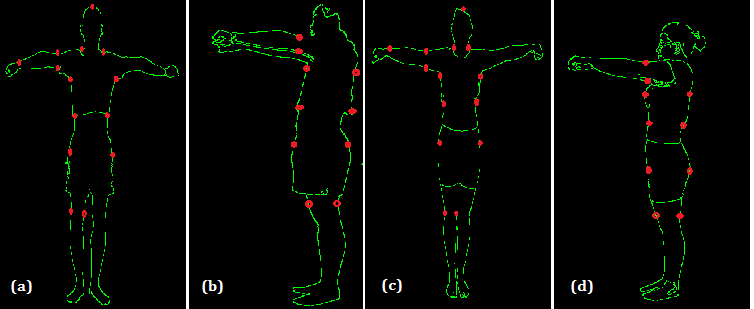
\includegraphics [scale=0.4] {images/h15.png}
\begin{center}
%\captionsetup{justification=justified, labelsep=period}
\caption{Результаты извелечения 12 антропометрических признаков} \label{img7}
\end{center}
\end{wrapfigure}
\textbf{Шаг 4:} Обнаружение контура и поиск ключевых точек признаков – алгоритм $ICP$. Используем соответствующее максимальное пороговое значение $d_{max}$. $d_{max}$ представляет собой баланс между сходимостью и точностью. Алгоритм $ICP$ повторяет действия, чтобы минимизировать среднеквадратичную ошибку пикселов, соответствующих ближайшей точке. $T\leftarrow argmin_t\left\{\sum_i\left\|T.b_i - m_i\right\|^2\right\}.$ Набор новых точек будет найден, если он удовлетворяет двум условиям: Расположен на границе или наиболее близко к границам объекта; Расстояние между двумя наборами точек считается наименьшим. Расчет евклидова расстояния: $d\left(A,B\right) = \sqrt{\left(x_B - x_A\right)^2 + \left(y_B - y_A\right)^2}$.

\textbf{Шаг 5:}Создание антропометрического вектора признаков

\textbf{Экспериментальное оценивание точности извлечения антропометрических признаков}. В этой части представлен результат извлечения антропометрических признаков на основе алгоритма компьютерного зрения с $50$ изображений. Такие изображения собраны автором. Извлечение признаков состоит из $2$ главных этапов: Предварительная обработка изображения, преобразование изображения в оттенках серого, фильтрация шумов, разряжение пикселей, балансировка гистограммы для получения лучшего качества изображения; Извлечение точек признаков с использованием алгоритма вычитания фона, обнаружения человеческого лица, сегментации изображения, поиска точек признаков. 
\begin{wrapfigure}{r}[0pt]{0.5\linewidth}
\centering
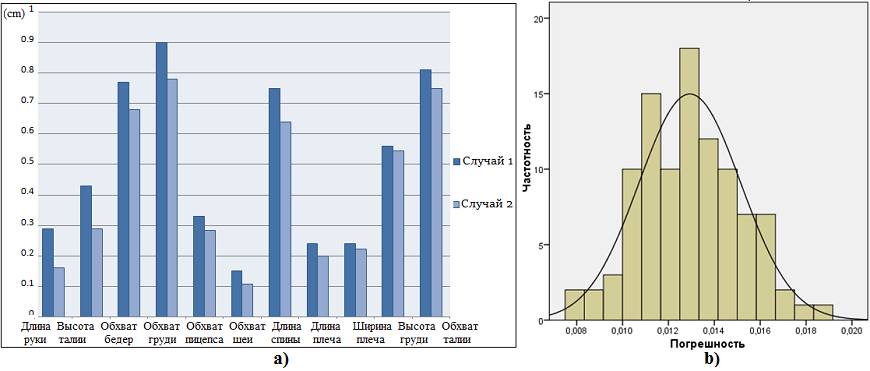
\includegraphics [scale=0.3] {images/h16.png}
\begin{center}
%\captionsetup{justification=justified, labelsep=period}
\caption{Погрешность разработанного метода антропометрии.} \label{img16}
\end{center}
\end{wrapfigure}
Для оценки эффективности процесса извлечения признаков применяются средняя абсолютная ошибка - $MAPE$. Она служит для оценки точности прогноза, показывает на сколько велики ошибки в сравнении со значениями ряда. Хороша для сравнения $1-й$ модели для разных рядов. Используется для сравнения разных моделей для одного ряда. Формула расчета $MAPE$: $M=\frac{1}{n}\sum^n_{i=1}\left|\frac{A_t-F_t}{A_t}\right|$, Где: $A_t$: Результат измерений, рассчитанных вручную; $F_t$: Результат извлечения антропометрических признаков.

\textbf {Приложение алгоритма Random Forest (случайного леса) для классификации антропометрических данных}
В данной работе предлагается алгоритм для оценки и поиска набора признаков из исходного набора атрибутов. Шаги выполнения алгоритма обозначается следующим образом:

\textbf{Шаг 1:} Создание $m$ наборов признаков из $n$ наборов первоначальных признаков. Каждый набор содержит $2 \frac{n}{m} $признаки. В том числе: $\frac{n}{m}$ признаки равны; $\frac{n}{m}$ случайные признаки.

\textbf{Шаг 2:} Использование Random Forest для того, чтобы вычислять оценку наборов признаков $\Rightarrow$ получение набора значений $f\left(i\right), i= \left(1,..., m\right)$;

\textbf{Шаг 3:}взвешивание каждого признака $i$ рассчитывается по формуле: $w_j= \sum^m_{i=1}kf_i$; $k_{ij} = 0$, если признак $i$ не выбран в наборе признака $j$; $k_{ij}= 1$, если признак выбран в наборе признака$j$.

\textbf{Шаг 4:} Разработка нового признака включает в себя $р\%$ лучших признаков;

\textbf{Шаг 5:} Повторение шага $1$ для удовлетворения одного из двух условий:  Количество признаков < порога разрешено; Количество циклов определено.

\textbf{Формирование опорных точек с признаками объектной принадлежности}. В этом разделе представлен подход к реконструкции 3D-модели человека \footnote{(С.Н. Грудинин - 2009), (С.Н. Грудинин -2014) предложен способ построения 3D-моделей на основе параметрического моделирования антропометрических характеристик человеческого тела.} на основе антропометрических признаков, которые были извлечены и классифицированы из 2D-изображений.
Мы используем набор данных  антропометрических признаков для построения 3D-модели точной и эффективной в соответствии с формой и фактическим размером объекта.
\begin{wrapfigure}{r}[0pt]{0.4\linewidth}
\centering
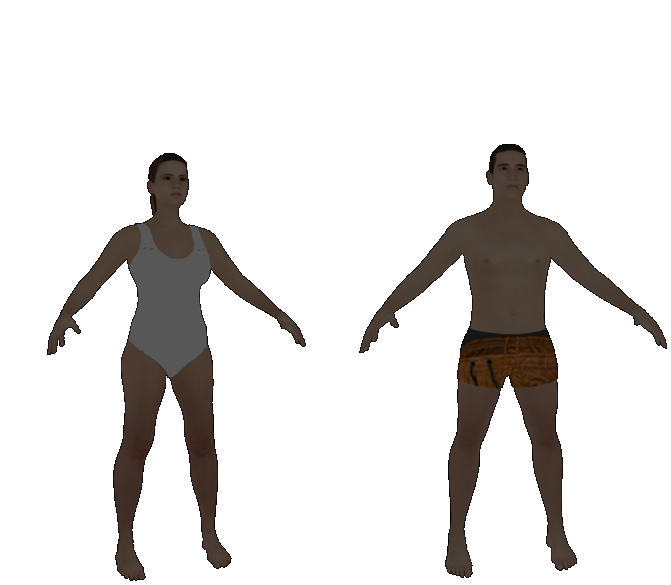
\includegraphics [scale=0.4] {images/h22.png}
\begin{center}
%\captionsetup{justification=justified, labelsep=period}
\caption{Результаты антропометрических моделей} \label{img17}
\end{center}
\end{wrapfigure}
Процесс построения антропометрических модели включает следующие шаги:

	\textbf{ Шаг 1}: Описание текстурных характеристик человеческого тела (кожа, волосы, лицо), а также текстуры одежды;
	
   \textbf{Шаг 2}: Разработка частей человеческого тела (голова, туловище, руки, ноги) с использованием ранее полученных антропометрических признаков;
	
\textbf{Шаг 3}: Комбинация текстуры и частей человеческого тела в блок;

\textbf{Шаг 4}: Экспорт антропометрических моделей человеческого тела в два файла: первый файл (*.mtl) описывает текстуры модели, второй файл (*.obj) содержает информацию каждой модели.

В \textbf {третьей главе} описывается анализ проектирования системы компьютерного зрения в антропометрии для практических применений: Текстильное приложение и фитнес-приложение. Система анализируется с помощью аналитических методов объектно-ориентированного UML. Программа описывается диаграммами: диаграмма прецедентов, диаграмма классов, диаграмма последовательности. Классы подробно анализируются, с указанием задач каждого компонента в программе. Также, в главе доказывается целесообразность проектирования приложений компьютерного зрения в антропометрии;
\begin{figure}[ht!]
\centering
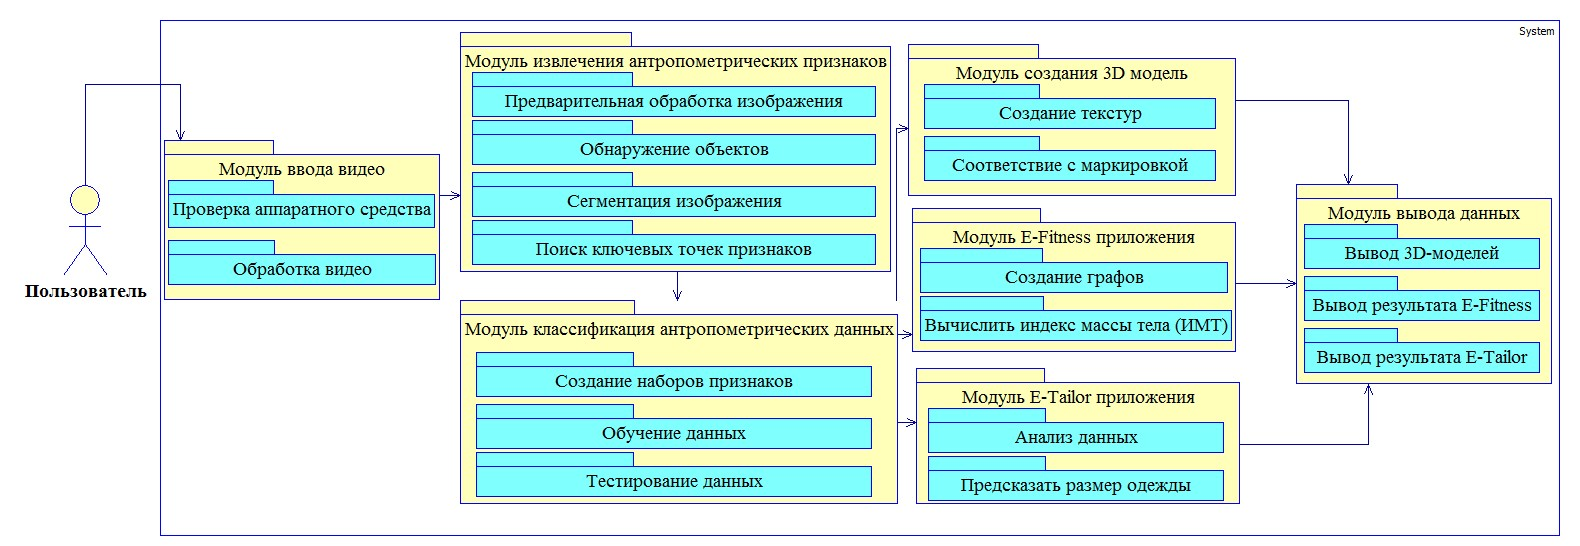
\includegraphics [scale=0.4] {images/h35.png}
\begin{center}
%\captionsetup{justification=justified, labelsep=period}
\caption{Структура ПО} \label{img35}
\end{center}
\end{figure}

Анализ практических результатов экспериментов периода извлечения антропометрических признаков. Сравнение результатов предложенных алгоритмов с другими алгоритмами по точности. Доказывается преимущество приведенного алгоритма на основе метода разреза на графах и итеративного алгоритма ближайших точек.

Сравнение результатов классификации между алгоритмом случайного леса и алгоритмом Boosting, работающими с видео, показало, что по точности и времени выполнения, более результативный алгоритм случайного леса для системы компьютерного зрения в антропометрии. Алгоритм случайного леса полностью совместим с визуальной системой.

В \textbf{четвертой главе} Описание среды разработки приложения Android, библиотек поддержки алгоритмов компьютерного зрения OpenCV, поддержки построения 3D-моделей человеческого тела MakeHuman и библиотеки поддержки 3D для Android – Min3D. Описание и инструкция для скачивания программы. Инструкция конфигурации библиотеки OpenCV с Android. Разработка приложения компьютерного зрения в антропометрии для пошива одежды (E-Tailor). Главные функции: автоматизация извлечения антропометрических признаков и классификация размеров одежды. Разработка приложения компьютерного зрения в антропометрии для фитнеса (E-Fitness). Главные функции: автоматизация извлечения антропометрических признаков, построение 3D-моделей человеческого тела, анализ и сравнение признаков по телосложению, индексу массы тела (ИМТ). Приложения разработаны на ОС Android для смартфонов и на основе методов и алгоритмов компьютерного зрения для извлечения и классификации антропометрических признаков. Программный модуль имеет простой, удобный и интуитивно понятный интерфейс.

\subsection*{ОСНОВНЫЕ РЕЗУЛЬТАТЫ ДИССЕРТАЦИОННОЙ РАБОТЫ}
В данной диссертации решены практические задачи научно-технических исследований и разработок алгоритмов компьютерного зрения в антропометрии на изображении и видео.

В диссертации выполнены работы и получены научно-практические результаты. Основные выводы заключаются в следующем:

\begin{enumerate}
	\item Исследование и разработка алгоритмов компьютерного зрения для  извлечения антропометрических признаков на изображении и видео, основанные на комбинации алгоритмов сегментации изображений разреза на графах (Graph-cuts) и итеративного алгоритма ближайших точек (ICP), построение множества ключевых точек объектов;
	\item Предложена модель и разработка алгоритма классификации данных методом случайного леса (Random Forest) для приложения, которое классифицирует объекты на основе антропометрических признаков;
	\item Разработка алгоритмов и методов компьютерного зрения в антропометрии на изображениях и видео с наличием шума и в режиме реального времени;
	\item Построение антропометрических 3D-моделей человеческого тела на основе результата извлечения антропометрических признаков;
	\item Развитие системы компьютерного зрения в антропометрии для смартфонов на ОС Android: приложение «E-Tailor» для текстильной промышленности и приложение «E-Fitness» для фитнеса.
\end{enumerate}



%{\textbf{Заключение.}}

%\input{../common/concl}
%%В данной работе рассмотрены интегральные ураневнения Вольтерра, особое место в которой занимает исследование численных методов решения уравнений Вольтерра первого рода с разрывными ядрами.
%%К необходимости поиска решений таких уравнений приводит задача моделирования стратегий развития электроэнергетических систем.
%%
%%Основные результаты работы заключаются в следующем.
%%\begin{enumerate}
	%%\item На основе анализа предметной области предложены новые методы построения численных решений интегральных уравнений Вольтерра первого рода с разрывными ядрами.
%%
	%%\item Приведены интегральные модели, описывающие практическое применение интегральных уравнений Вольтерра первого рода с разрывными ядрами, и методы прогнозирования %параметров ЭЭС.
%%спада использования энергии для ее сбережения и последующего использования при пиковой нагрузке.
%%
	%%\item Разработан для выполнения поставленных задач новый проблемно-ориентированный программный комплекс для моделирования развивающихся ЭЭС для возможности построения математических моделей развивающихся динамических систем на основе интегральных уравнений Вольтерра первого рода с разрывными ядрами с использованием квадратурных формул средних прямоугольников при различных аппроксимациях искомого решения. 
%%
	%%\item Численные исследования показали, что предложенные алгоритмы достаточно эффективны для решения поставленных задач.
%%
%%\end{enumerate}
%%
%%В качестве дальнейшего направления работы можно обозначить исследования устойчивости численных методов решения уравнений Вольтерра первого рода с разрывными ядрами, разработку программного обеспечения для моделирования реальных практических задач, а также использование моделей, описываемых рассматриваемыми уравнениями, не только в энергетической отрасли, но и в других областях.

%В данной работе рассмотрены интегральные уравнения, особое место в которой занимает исследование численных методов решения уравнений Вольтерра первого рода с разрывными ядрами.
%К необходимости поиска решений таких уравнений приводит задача моделирования стратегий %развития электроэнергетических систем.
%использования дополнительных генерирующих мощностей на основе %энергосберегающих технологий
%технологий аккумулирования электроэнергии, с тем чтобы покрыть пиковый спрос потребителей в электроэнергии
%
%Основные результаты работы заключаются в следующем.
%\begin{enumerate}
	%\item На основе анализа предметной области предложены новые методы построения численных решений интегральных уравнений Вольтерра первого рода с разрывными ядрами.
%
	%\item Приведены интегральные модели, описывающие практическое применение интегральных уравнений Вольтерра первого рода, и методы, %прогнозирования параметров ЭЭС.
%которые позволяют найти эффективный алгоритм задействования дополнительных мощностей для покрытия пика потребления электроэнергии.
%
	%\item Разработан для выполнения поставленных задач новый проблемно-ориентированный программный комплекс для 
	%%моделирования развивающихся ЭЭС 
	%проведения детального анализа развития динамических систем с учетом %старения оборудования, 
 %задействования %дополнительных мощностей %энергосберегающих технологий при заранее известном прогнозе потребления
%%с использованием 
%различных видов 
%%накопителей энергии при
%технологий аккумулирования электроэнергии при заранее известном прогнозе потребления
	%%для возможности построения математических моделей развивающихся динамических систем 
	%на основе интегральных уравнений Вольтерра первого рода с разрывными ядрами с использованием квадратурных формул средних прямоугольников и Гаусса при различных аппроксимациях искомого решения. 
%
	%\item Численные исследования показали, что предложенные алгоритмы достаточно эффективны для решения поставленных задач.
%
%\end{enumerate}
%
%В качестве дальнейшего направления работы можно обозначить исследования устойчивости численных методов решения уравнений Вольтерра первого рода с разрывными ядрами, разработку программного обеспечения для моделирования реальных практических задач для отраслей отечественной промышленности, а также использование моделей, описываемых рассматриваемыми уравнениями, не только в энергетической отрасли, но и в других областях.


%\newpage
%\renewcommand{\refname}{\large Публикации автора по теме диссертации}

%\nocite{*}
%\insertbiblioauthor                          % Подключаем Bib-базы
%%%%%%\insertbibliofull
%
%
%\renewcommand{\refname}{{\large Публикации по теме диссертации}\\
%{\normalsize\textnormal{Публикации в изданиях из перечня ВАК:}}}
%
%\renewcommand{\refname}{\normalsize\textnormal{Публикации в других изданиях:}}
%\insertbibliononvak